%----------------------------------------------------------------------------------------
%    PACKAGES AND THEMES
%----------------------------------------------------------------------------------------

\documentclass[aspectratio=169,xcolor=dvipsnames]{beamer}
\usetheme{SimpleDarkBlue}

\usepackage{hyperref}
\usepackage{graphicx} % Allows including images
\usepackage{booktabs} % Allows the use of \toprule, \midrule and \bottomrule in tables

\usepackage{caption} % Allows the usage of \captionsetup
\DeclareCaptionFormat{nolabel}{#3} % Removes "Listing:" prefix
\captionsetup[lstlisting]{format=nolabel}

\usepackage{enumitem}
\setlist[itemize,1]{label=\textbullet}
\setlist[itemize,2]{label=--}

\usepackage[T1]{fontenc}
\usepackage{cascadia-code}

\usepackage{xcolor}
\definecolor{codegreen}{rgb}{0,0.6,0}
\definecolor{codegray}{rgb}{0.5,0.5,0.5}
\definecolor{codepurple}{rgb}{0.58,0,0.82}
\definecolor{backcolour}{rgb}{0.9,0.9,0.9}

\usepackage{listings}
\lstdefinestyle{mystyle}{
    backgroundcolor=\color{backcolour},
    commentstyle=\color{codegreen},
    keywordstyle=\color{magenta},
    numberstyle=\tiny\color{codegray},
    stringstyle=\color{codepurple},
    basicstyle=\ttfamily\footnotesize,
    breakatwhitespace=false,
    breaklines=true,
    captionpos=b,
    keepspaces=true,
    numbers=left,
    numbersep=5pt,
    showspaces=true,
    showstringspaces=true,
    showtabs=true,
    tabsize=4,
    aboveskip=0pt, % Reduce space above
    belowskip=0pt  % Reduce space below
}
\lstset{style=mystyle}

%----------------------------------------------------------------------------------------
%    TITLE PAGE
%----------------------------------------------------------------------------------------

\title{Ateliers Créactifs Raspberry Pi}
\subtitle{Hébergement de son propre système multimédia avec Jellyfin}

\author{Jean Bourgies, François Marelli, Ugo Proietti}

\date{7 avril 2025}

%----------------------------------------------------------------------------------------
%    PRESENTATION SLIDES
%----------------------------------------------------------------------------------------

\begin{document}

\begin{frame}
    % Print the title page as the first slide
    \titlepage
\end{frame}

\begin{frame}{Table des matières}
    % Throughout your presentation, if you choose to use \section{} and \subsection{} commands, these will automatically be printed on this slide as an overview of your presentation
    \tableofcontents
\end{frame}


%------------------------------------------------
\section{Gestion des fichiers/dossiers sur Linux}
%------------------------------------------------

\begin{frame}{Lister les blocs de stockage}
    \begin{columns}[c] % 'c' ensures vertical centering for both columns

        \column{1\textwidth}
        \begin{itemize}
            \item \texttt{lsblk} est un outil pour lister les blocs de stockage.
        \end{itemize}
        \begin{figure}
            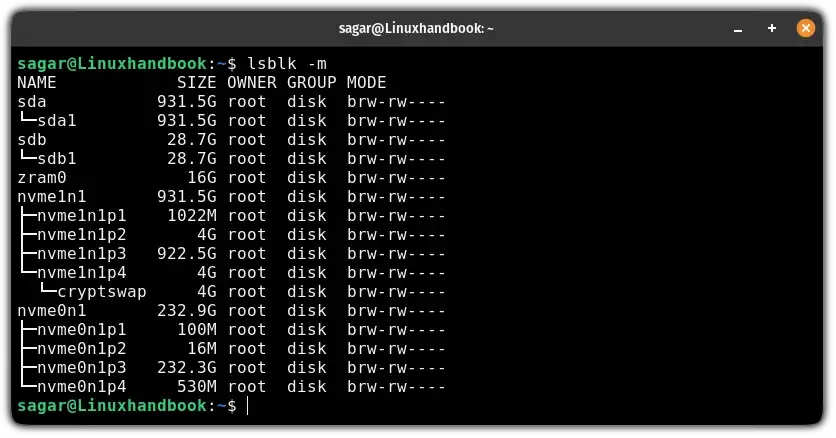
\includegraphics[width=0.7\textwidth]{images/lsblk.png}
        \end{figure}

    \end{columns}
\end{frame}

\begin{frame}{Partitioner un disque}
    \begin{columns}[c] % 'c' ensures vertical centering for both columns

        \column{1\textwidth}
        \begin{itemize}
            \item \texttt{cfdisk}, \texttt{parted}, \texttt{fdisk} sont des outils pour partioner des disques.
        \end{itemize}
        \begin{figure}
            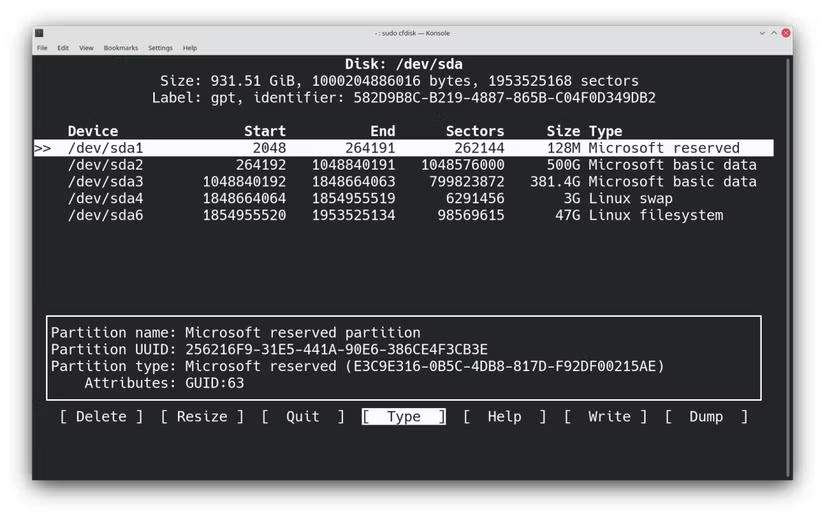
\includegraphics[width=0.7\textwidth]{images/cfdisk.png}
        \end{figure}

    \end{columns}
\end{frame}

\begin{frame}{Formater une partition}
    \begin{columns}[c] % 'c' ensures vertical centering for both columns

        \column{1\textwidth}
        \begin{itemize}
            \item Pour formater en ext4 (utilisé sur Linux)
            \begin{itemize}
                \item \texttt{sudo mkfs.ext4 /dev/sdX1}
            \end{itemize}
            \item Pour formater en NTFS (utilisé sur Windows et compatible avec Linux)
                \begin{itemize}
                    \item \texttt{sudo apt install ntfs-3g}
                    \item \texttt{sudo mkfs.ntfs /dev/sdX1}
                \end{itemize}
        \end{itemize}

    \end{columns}
\end{frame}

\begin{frame}{Monter et démonter du stockage externe}
    \begin{columns}[c] % 'c' ensures vertical centering for both columns

        \column{1\textwidth}
        \begin{itemize}
            \item Créer au préalable un dossier où monter le contenu de la clé USB :
            \begin{itemize}
                \item \texttt{mkdir /mnt/macleusb}
            \end{itemize}
            \item Pour le montage :
            \begin{itemize}
                \item \texttt{sudo mount /dev/sdX /mnt/macleusb}
            \end{itemize}
            \item Pour le montage :
            \begin{itemize}
                \item \texttt{sudo umount /mnt/macleusb}
            \end{itemize}
        \end{itemize}

    \end{columns}
\end{frame}

\begin{frame}{Gestion des permissions}
    \begin{columns}[c] % 'c' ensures vertical centering for both columns

        \column{1\textwidth}
        \begin{itemize}
            \item La commande \texttt{chmod} permet de changer les permission d'un fichier ou d'un dossier.
            \begin{itemize}
                \item \texttt{sudo chmod 777 /home/ugo/Documents/presentation.pdf}
            \end{itemize}
        \end{itemize}

        \begin{columns}[c] % 'c' ensures vertical centering for both columns
            \column{0.7\textwidth}
            \begin{figure}
                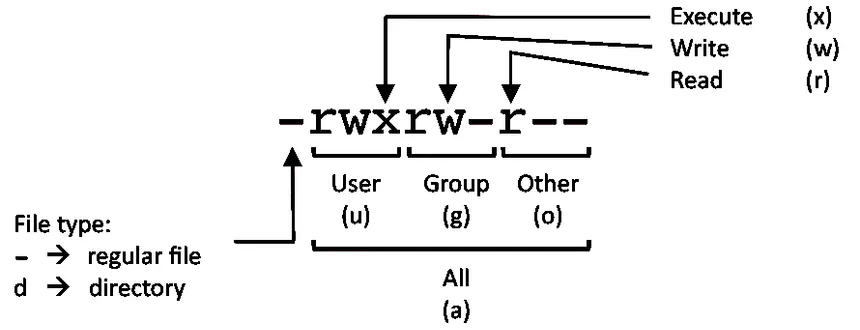
\includegraphics[width=1\textwidth]{images/chmod.png}
            \end{figure}

            \column{0.3\textwidth}
            \begin{table}[]
            \begin{tabular}{|l|l|}
            \hline
            0 & - - - \\ \hline
            1 & - - x \\ \hline
            2 & - w - \\ \hline
            3 & - w x \\ \hline
            4 & r - - \\ \hline
            5 & r - x \\ \hline
            6 & r w - \\ \hline
            7 & r w x \\ \hline
            \end{tabular}
            \end{table}
        \end{columns}
    \end{columns}
\end{frame}

%------------------------------------------------
\section{Besoins matériel}
%------------------------------------------------

\begin{frame}{Jellyfin sur la carte Raspberry Pi}
    \begin{columns}[c] % 'c' ensures vertical centering for both columns

        \column{1\textwidth}
        \begin{itemize}
            \item Peu adapté.
            \item Performances assez faibles en 4K.
            \item Accélération matérielle peu compatible et donc mauvais transcodage.
        \end{itemize}

    \end{columns}
\end{frame}

\begin{frame}{Carte SD}
    \begin{columns}[c] % 'c' ensures vertical centering for both columns

        \column{1\textwidth}
        \begin{itemize}
            \item À éviter.
            \item Performances moins bonnes que celles d'un SSD.
            \begin{itemize}
                \item En lecture : Environ 40MB/s pour la SD contre environ 500MB/s pour le SSD.
            \end{itemize}
            \item Usure due au cache du transcodage.
        \end{itemize}

    \end{columns}
\end{frame}

%------------------------------------------------
\section{Installation de Jellyfin}
%------------------------------------------------

\begin{frame}{Jellyfin}
    \begin{columns}[c] % 'c' ensures vertical centering for both columns

        \column{1\textwidth}
        \begin{itemize}
            \item \url{https://jellyfin.org/}
            \item \url{https://demo.jellyfin.org}
        \end{itemize}

    \end{columns}
\end{frame}

\end{document}
